\documentclass[11pt,a4paper]{article}
\usepackage[utf8]{inputenc}
\usepackage[T1]{fontenc}
\usepackage[spanish,es-noshorthands]{babel}
\usepackage[margin=2.3cm]{geometry}
\usepackage{graphicx}
\usepackage{array}
\usepackage{url}

\setlength{\parskip}{4pt}
\setlength{\parindent}{0pt}
\renewcommand{\arraystretch}{1.15}
\newcommand{\code}[1]{\texttt{#1}}

\begin{document}

% ====================== PORTADA ======================
\begin{titlepage}
\centering
\vspace*{1.5cm}
{\large Universidad Tecnológica Metropolitana (UTEM)\par}
{\large Procesamiento Digital de la Información --- INFB6073\par}
\vspace{2.2cm}
{\Huge\bfseries Diseño y Evaluación Experimental de un\\[4pt] Sistema de Conteo Automático de Monedas\par}
\vspace{0.6cm}
{\large\itshape Informe Técnico --- Tarea 2\par}
\vspace{2.5cm}
\begin{tabular}{rl}
\textbf{Autor:} & Francisco Alejandro Pinto Abraham\\
\textbf{RUT:} & 21.571.239-7\\
\textbf{Profesor:} & Jorge R. Vergara\\
\textbf{Semestre:} & Primer semestre 2026\\
\end{tabular}
\vfill
{\small Código y datos: \url{https://github.com/k0ngan/monedas}\par}
{\small Junio de 2026\par}
\end{titlepage}

% ====================== 1. INTRODUCCION ======================
\section{Introducción}

El conteo automático de objetos es un problema clásico de visión por computador con aplicaciones directas
en automatización bancaria y financiera. A pesar del auge del aprendizaje profundo, las \textbf{técnicas
clásicas} de procesamiento digital de imágenes siguen siendo atractivas por su interpretabilidad, su bajo
coste computacional y su facilidad de implementación en sistemas con recursos limitados.

Este informe aborda la construcción y evaluación de un sistema de \textbf{conteo automático de monedas
japonesas (yen)} utilizando \emph{exclusivamente} los métodos revisados durante el curso (Colabs de
clase). El núcleo del sistema es el procedimiento que el profesor presentó para contar monedas (Clase~16):
conversión a gris con realce de intensidad, umbralización, morfología matemática, etiquetado de
componentes conexas y filtrado de las regiones por sus propiedades de forma (área y excentricidad),
finalizando con la localización mediante \emph{bounding boxes}. Como segunda estrategia de segmentación se
emplea \textbf{k-means} de color (Clase~15) y, para el análisis espacio--frecuencia, la \textbf{Transformada
de Fourier 2D} (\code{scipy.fft}, Clases 05--10). No se utilizan watershed, transformada de Hough ni CLAHE
por no haber sido revisados en clase.

\textbf{Base de datos.} Se trabaja con un subconjunto curado de \textbf{26 fotografías yen} (120 monedas en
total) de la base pública de monedas, seleccionadas para cubrir distintos niveles de dificultad:
variaciones de resolución (de $\sim$0{,}25 a $\sim$12~MP), iluminación (escenas oscuras y saturadas),
contraste, fondos y \textbf{superposición} entre monedas. Se descartaron deliberadamente las
miniaturas/infografías con texto superpuesto, que no son fotografías reales de monedas y generan
detecciones espurias. El conteo real de cada imagen (\emph{ground truth}) se conoce y se usa para evaluar.

\textbf{Objetivo.} Más allá de obtener un algoritmo que cuente monedas, el estudio busca \emph{analizar
críticamente} el problema, comparar alternativas metodológicas y justificar las decisiones técnicas con
evidencia experimental.

% ====================== 2. METODOS ======================
\section{Descripción de los métodos y algoritmos}

La cadena de procesamiento propuesta, desde la imagen original hasta la estimación del número de monedas,
se resume en el diagrama de la Figura~\ref{fig:diagrama}.

\begin{figure}[ht]
\centering
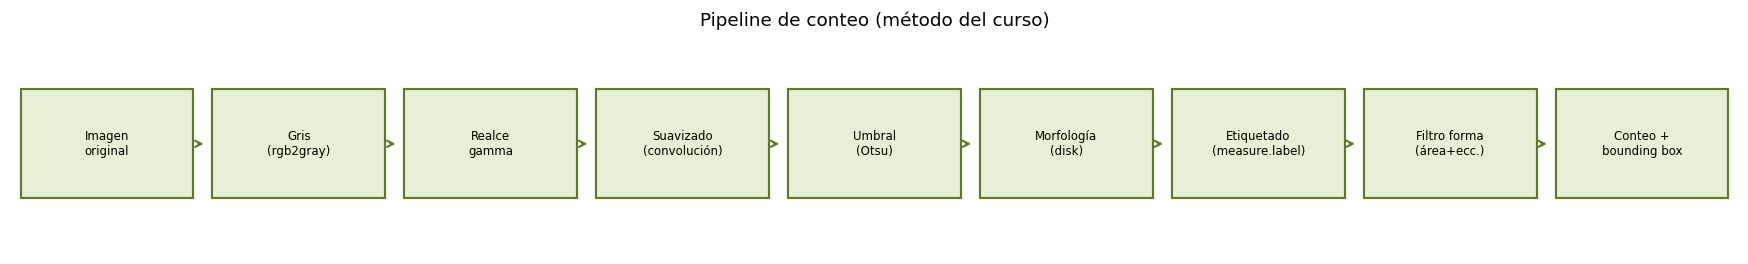
\includegraphics[width=\linewidth]{figs/diagrama.png}
\caption{Diagrama de bloques del sistema de conteo (método del curso).}
\label{fig:diagrama}
\end{figure}

\textbf{Etapas y su justificación} (entre paréntesis, el Colab de clase que introduce cada técnica):

\begin{itemize}
\item \textbf{Escala de grises} con \code{color.rgb2gray}: reduce a un canal de intensidad; el color no
aporta a la segmentación de monedas metálicas.
\item \textbf{Realce gamma} $g^{\gamma}$ con $\gamma=0{,}6$ (Clase~16): aclara las zonas oscuras y mejora
el bajo contraste antes de umbralizar.
\item \textbf{Suavizado} por convolución (\code{gaussian\_filter}, $\sigma=1$; Clase~16-06-02): atenúa
ruido y reflejos para evitar bordes falsos.
\item \textbf{Umbralización de Otsu} (\code{filters.threshold\_otsu}): obtiene un umbral global óptimo de
forma automática, con corrección de polaridad (se asume que el borde de la imagen es fondo).
\item \textbf{Morfología} con elemento estructurante \code{morphology.disk} y operaciones de apertura y
cierre (Clase~16): elimina motas y rellena huecos, dejando una máscara limpia.
\item \textbf{Etiquetado de componentes conexas} con \code{measure.label} (Clase~16): asigna una etiqueta
a cada región conectada de la máscara.
\item \textbf{Filtro de forma} con \code{measure.regionprops} (Clase~16): conserva solo las regiones con
\emph{área} suficiente ($\ge 0{,}08\%$ del cuadro) y \emph{excentricidad} baja ($\le 0{,}92$), descartando
ruido y blobs alargados producto de fusiones; el número de regiones que sobreviven es el conteo estimado.
\item \textbf{Localización} con \code{region.bbox} y \code{matplotlib.patches.Rectangle}: dibuja la caja de
cada moneda detectada.
\end{itemize}

La Figura~\ref{fig:pipeline} muestra la salida visual de cada transformación sobre una imagen de ejemplo,
incluyendo las cajas de detección.

\begin{figure}[ht]
\centering
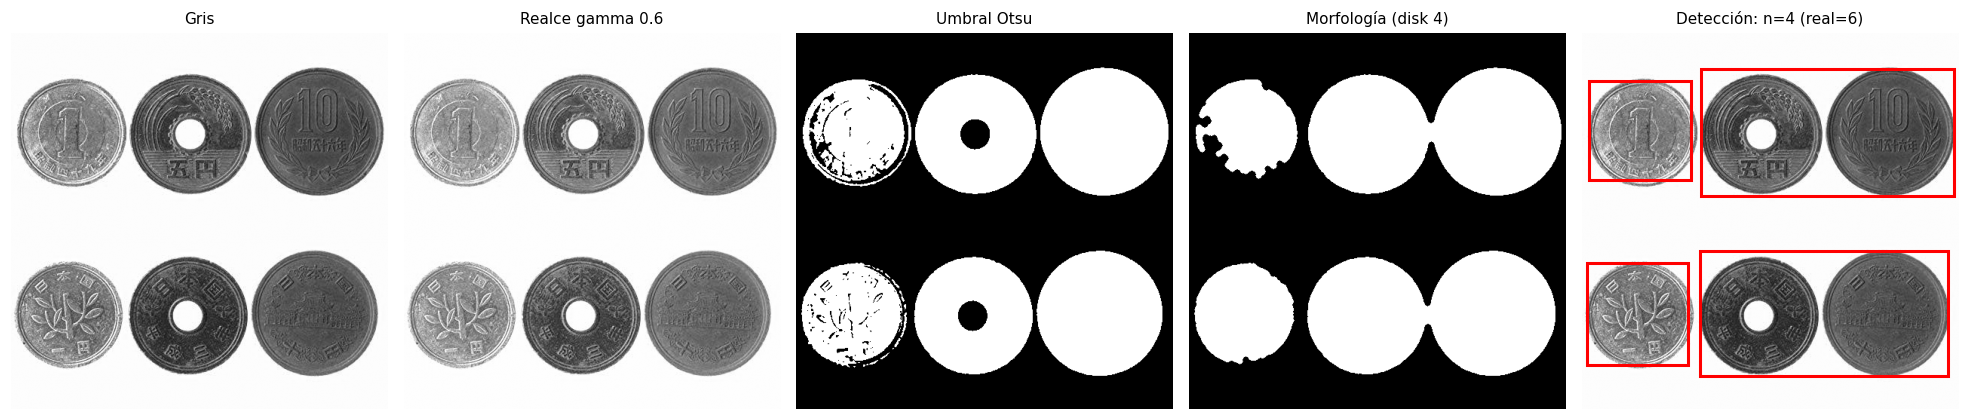
\includegraphics[width=\linewidth]{figs/pipeline_bbox.png}
\caption{De izquierda a derecha: gris, realce gamma, umbral de Otsu, morfología y detección final con
\emph{bounding boxes} (estimación $n=6$ sobre 6 monedas reales).}
\label{fig:pipeline}
\end{figure}

\textbf{Configuraciones evaluadas (Parte III).} Se comparan tres configuraciones, todas con técnicas del
curso, que difieren en la estrategia de segmentación o detección:
\begin{itemize}
\item \textbf{C1 --- Etiquetado simple:} gamma $\rightarrow$ Otsu $\rightarrow$ morfología $\rightarrow$
\code{label} $\rightarrow$ filtro de \emph{área}.
\item \textbf{C2 --- Etiquetado + forma (método del profesor):} añade el filtro de \emph{excentricidad}.
\item \textbf{C3 --- Segmentación por k-means:} \code{KMeans} sobre el color separa moneda/fondo, luego
\code{label} y los mismos filtros.
\end{itemize}

\textbf{Métodos de detección (Parte IV).} Se comparan dos estrategias \emph{revisadas en clase}: (A)
\textbf{componentes conexas + bounding boxes} (\code{measure.label}+\code{regionprops}) y (B)
\textbf{segmentación por k-means} de color. No se incluye la transformada de Hough: aunque el enunciado la
menciona como ejemplo, exige técnicas ``revisadas durante el curso'' y Hough no aparece en ningún Colab.

% ====================== 3. RESULTADOS ======================
\section{Resultados}

\subsection{Caracterización de los datos (Parte I)}

La Tabla~\ref{tab:stats} reporta, para 10 imágenes representativas, la resolución espacial y las
intensidades (mínima, máxima, media y desviación estándar). La Figura~\ref{fig:grid} las muestra y la
Figura~\ref{fig:histos} presenta cinco histogramas.

\begin{table}[ht]
\centering
\small
\caption{Métricas de las 10 imágenes representativas (intensidades sobre escala de grises 0--255).}
\label{tab:stats}
\begin{tabular}{lcccccc}
\hline
Imagen & Monedas & Resolución & Int.\ mín & Int.\ máx & Media & Desv.\ est. \\
\hline
af8934a76c & 1  & 1300$\times$1117 & 0  & 255 & 186.8 & 81.6 \\
bead3b82b7 & 1  & 573$\times$591   & 32 & 255 & 209.5 & 39.5 \\
83dce1fa00 & 2  & 612$\times$416   & 73 & 255 & 224.8 & 31.5 \\
813563c984 & 2  & 4032$\times$3024 & 0  & 255 & 35.3  & 59.9 \\
c6e61445d9 & 3  & 612$\times$408   & 0  & 254 & 37.9  & 30.7 \\
232c6beb27 & 5  & 3366$\times$2192 & 0  & 255 & 68.9  & 87.8 \\
8eb878ba2e & 12 & 1300$\times$1068 & 0  & 255 & 209.6 & 47.4 \\
01685f1057 & 7  & 1300$\times$956  & 0  & 255 & 112.0 & 74.9 \\
858451585d & 9  & 1300$\times$956  & 0  & 255 & 120.5 & 77.1 \\
1c1c268cb8 & 14 & 1300$\times$956  & 0  & 255 & 174.0 & 62.2 \\
\hline
\end{tabular}
\end{table}

\begin{figure}[ht]
\centering
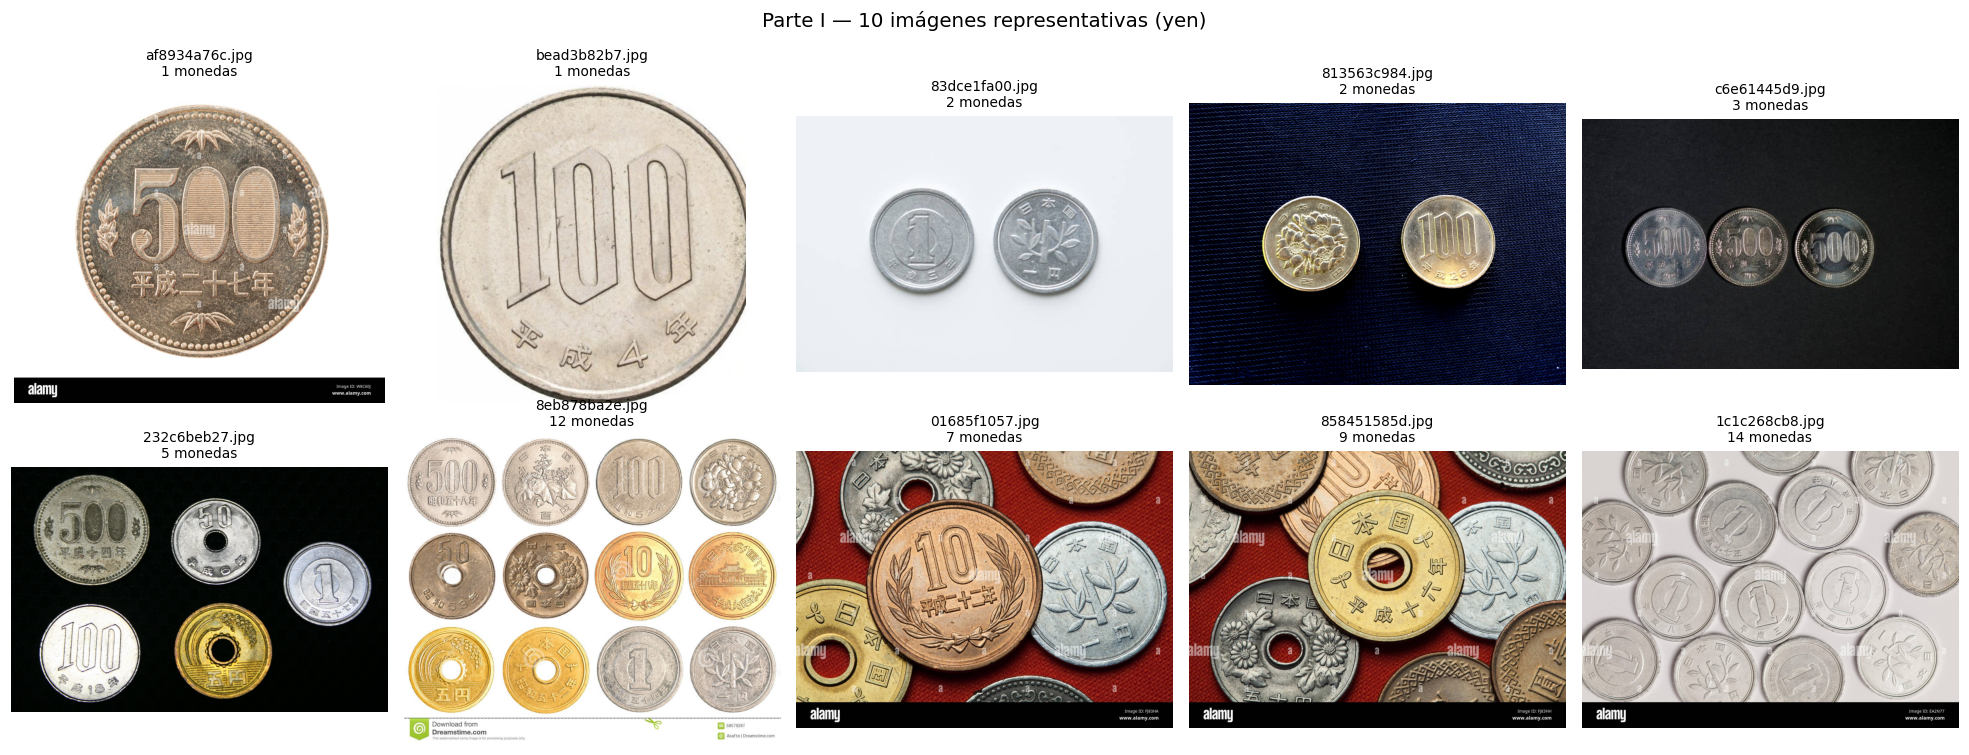
\includegraphics[width=\linewidth]{figs/grid.png}
\caption{Las 10 imágenes representativas, con distinto número de monedas, resolución, iluminación y grado
de solapamiento.}
\label{fig:grid}
\end{figure}

\begin{figure}[ht]
\centering
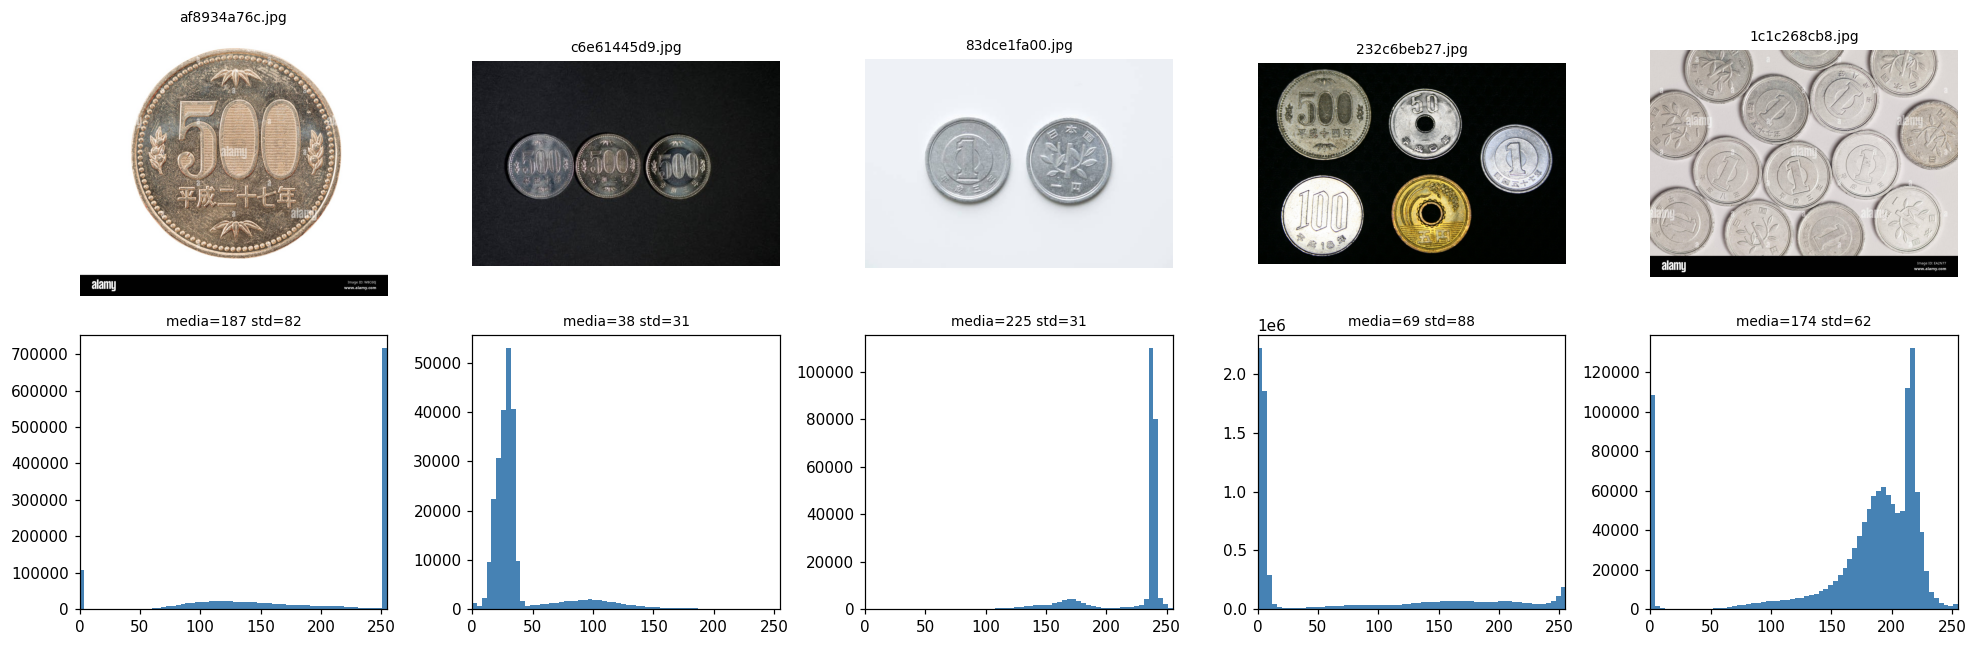
\includegraphics[width=\linewidth]{figs/histos.png}
\caption{Histogramas de cinco imágenes. Alto contraste: \code{232c6beb27}, \code{af8934a76c} (amplios y
bimodales). Bajo contraste / iluminación problemática: \code{c6e61445d9} (oscura) y \code{83dce1fa00}
(saturada). Segmentación compleja: \code{1c1c268cb8} (plata, monedas en contacto).}
\label{fig:histos}
\end{figure}

Del análisis de los histogramas se desprende que un histograma \textbf{bimodal con valle profundo} es la
condición ideal para Otsu, mientras que los histogramas unimodales y sesgados (escenas oscuras o saturadas)
anticipan las imágenes difíciles. El histograma, además, \emph{pierde la información espacial}, lo que
justifica complementar la umbralización con morfología y etiquetado. La Figura~\ref{fig:factores} ilustra
tres factores de dificultad presentes en la base de datos.

\begin{figure}[ht]
\centering
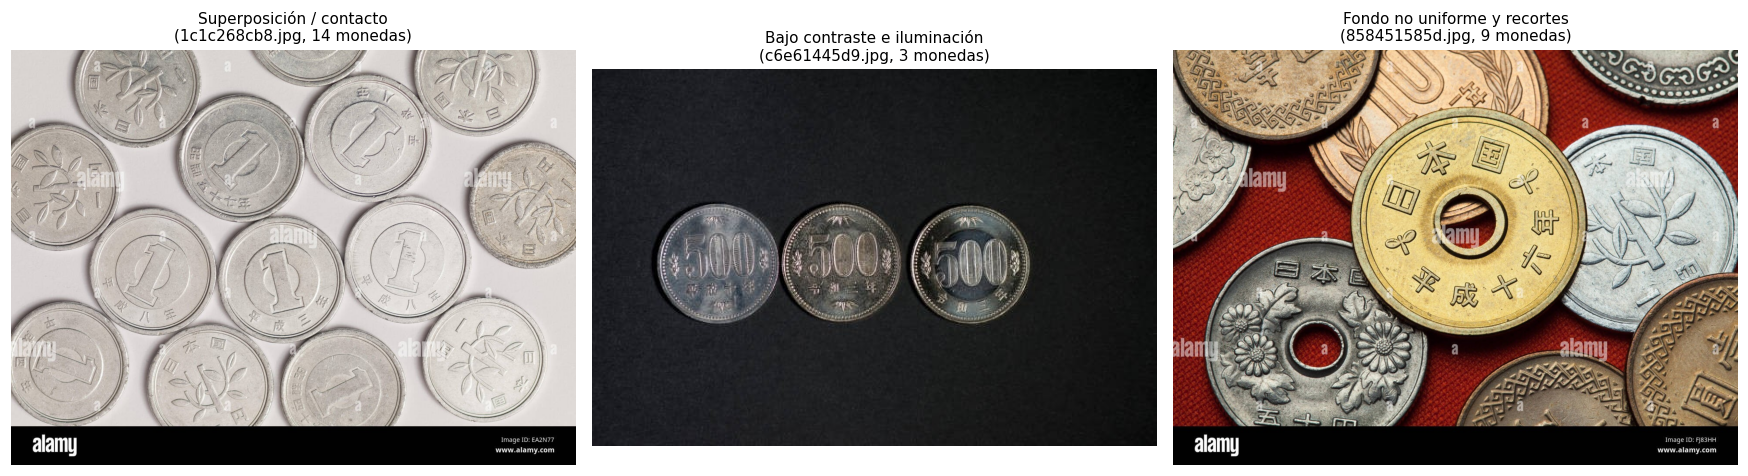
\includegraphics[width=\linewidth]{figs/factores.png}
\caption{Factores que dificultan el conteo: superposición/contacto, bajo contraste e iluminación
deficiente, y fondo no uniforme con monedas recortadas.}
\label{fig:factores}
\end{figure}

\subsection{Evaluación de las configuraciones (Parte III)}

Cada configuración se aplicó a las \textbf{26 imágenes}, reportando el conteo real, el estimado y el error
absoluto. La Tabla~\ref{tab:resumen} resume el desempeño y la Figura~\ref{fig:barras} lo grafica.

\begin{table}[ht]
\centering
\caption{Desempeño por configuración sobre las 26 imágenes. MAE = error absoluto medio.}
\label{tab:resumen}
\begin{tabular}{lccccc}
\hline
Configuración & MAE & Error total & Exactas (\%) & $\pm$1 (\%) & Tiempo (ms) \\
\hline
C1 etiquetado        & 1.65 & 43 & 42.3 & 65.4 & 480.5 \\
C2 +excentricidad    & 1.69 & 44 & 42.3 & 61.5 & 359.8 \\
\textbf{C3 k-means}  & \textbf{1.50} & \textbf{39} & \textbf{50.0} & \textbf{69.2} & 513.6 \\
\hline
\end{tabular}
\end{table}

\begin{figure}[ht]
\centering
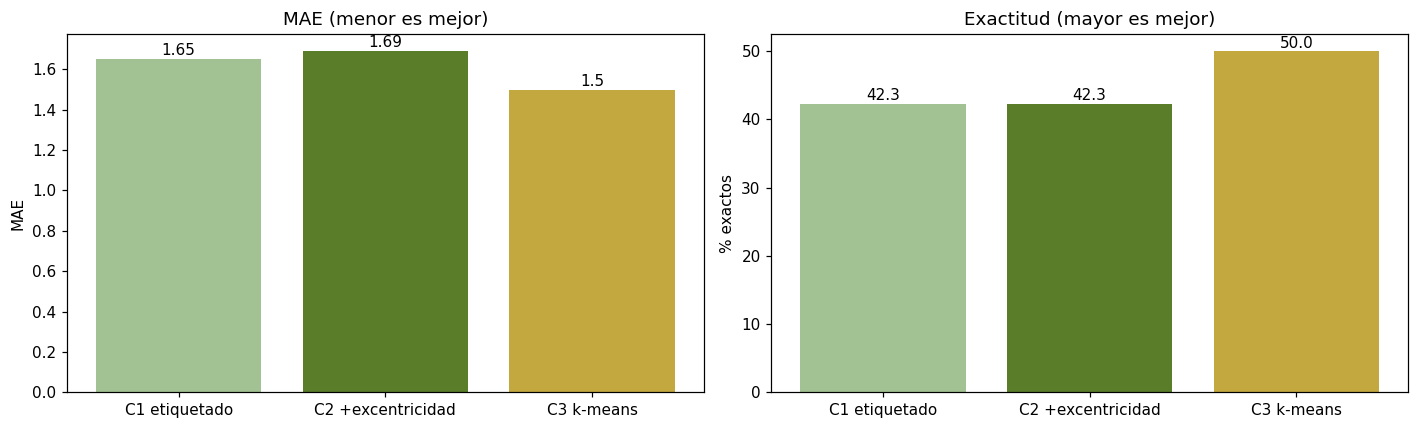
\includegraphics[width=0.95\linewidth]{figs/barras.png}
\caption{MAE (menor es mejor) y porcentaje de conteos exactos (mayor es mejor) por configuración.}
\label{fig:barras}
\end{figure}

La Figura~\ref{fig:casos} muestra tres casos exitosos y tres fallidos de C2 con sus cajas de detección.

\begin{figure}[ht]
\centering
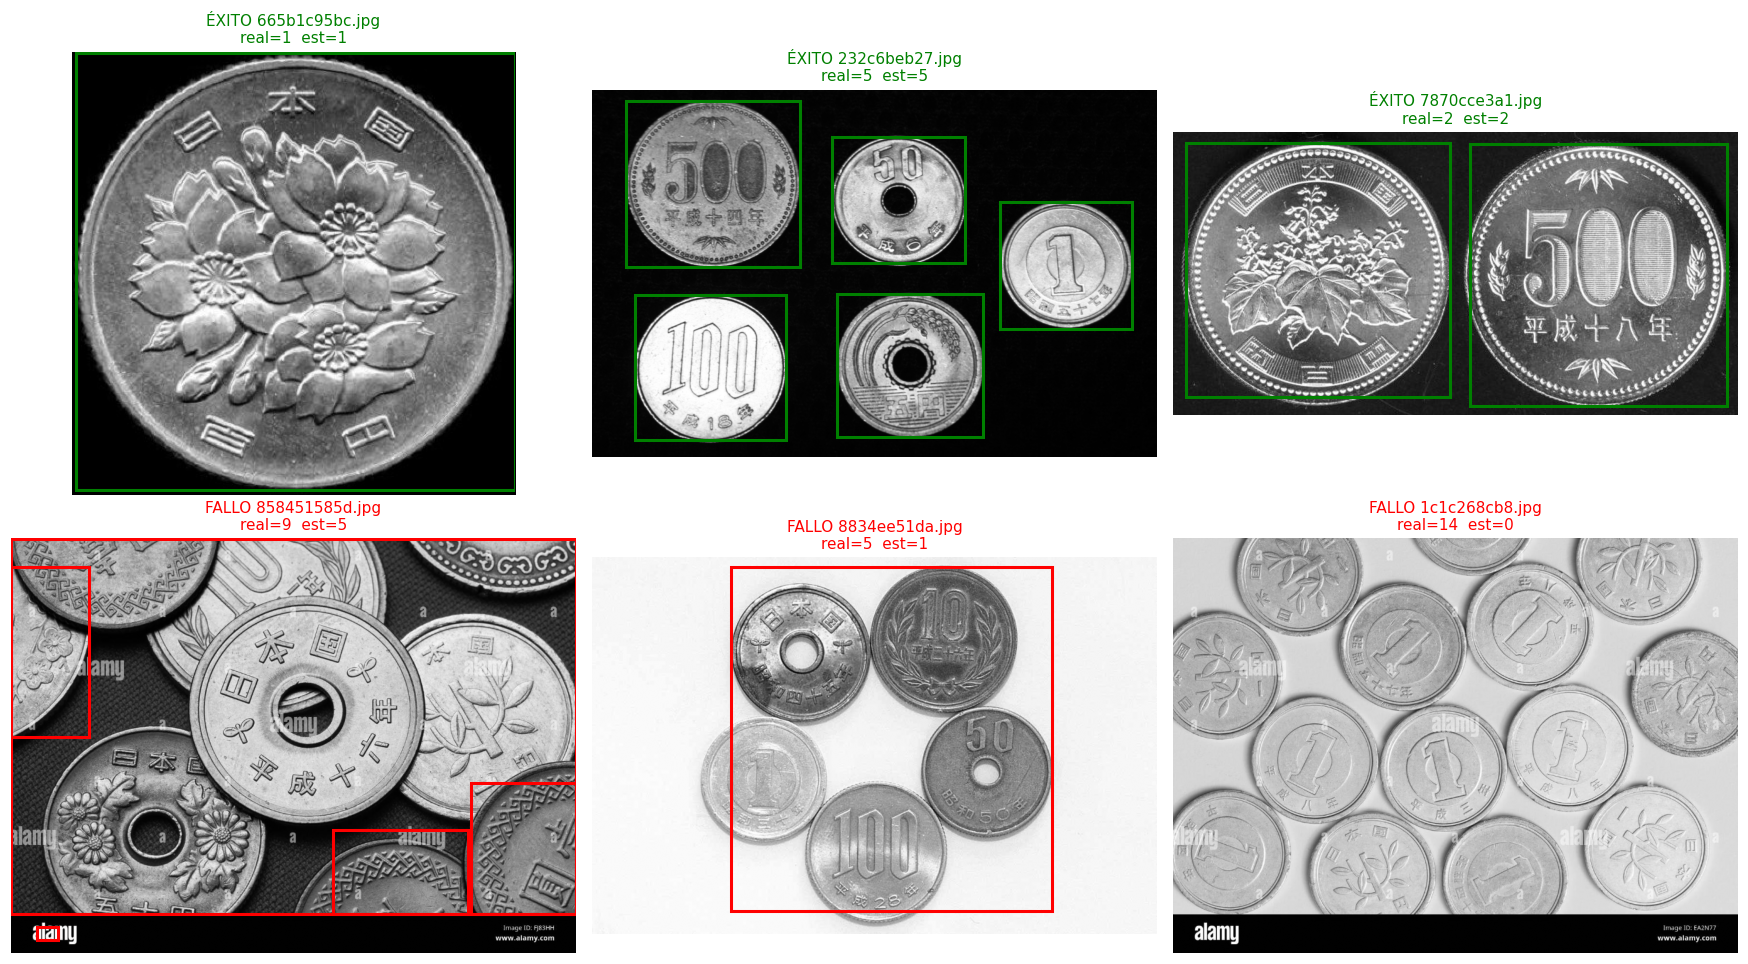
\includegraphics[width=\linewidth]{figs/exitos_fallos.png}
\caption{Casos exitosos (arriba) y fallidos (abajo) de la configuración C2.}
\label{fig:casos}
\end{figure}

\subsection{Comparación de métodos de detección (Parte IV)}

\begin{table}[ht]
\centering
\small
\caption{Comparación experimental de los dos métodos de detección.}
\label{tab:deteccion}
\begin{tabular}{lcccccc}
\hline
Método & MAE & Exactas (\%) & Tiempo (ms) & Robustez ilum. & Sensibilidad & Coste \\
\hline
Componentes + bbox (C2) & 1.69 & 42.3 & 359.8 & media & media (área, ecc., disk) & bajo \\
k-means (C3)            & 1.50 & 50.0 & 513.6 & media-alta & alta ($k$, semilla) & alto \\
\hline
\end{tabular}
\end{table}

\subsection{Relación espacio--frecuencia (Parte V)}

La Figura~\ref{fig:fourier} muestra los espectros de Fourier (\code{scipy.fft.fft2}+\code{fftshift}) de una
imagen con resultado correcto y otra con error, y la Figura~\ref{fig:sobel} el realce de bordes por
convolución (Sobel).

\begin{figure}[ht]
\centering
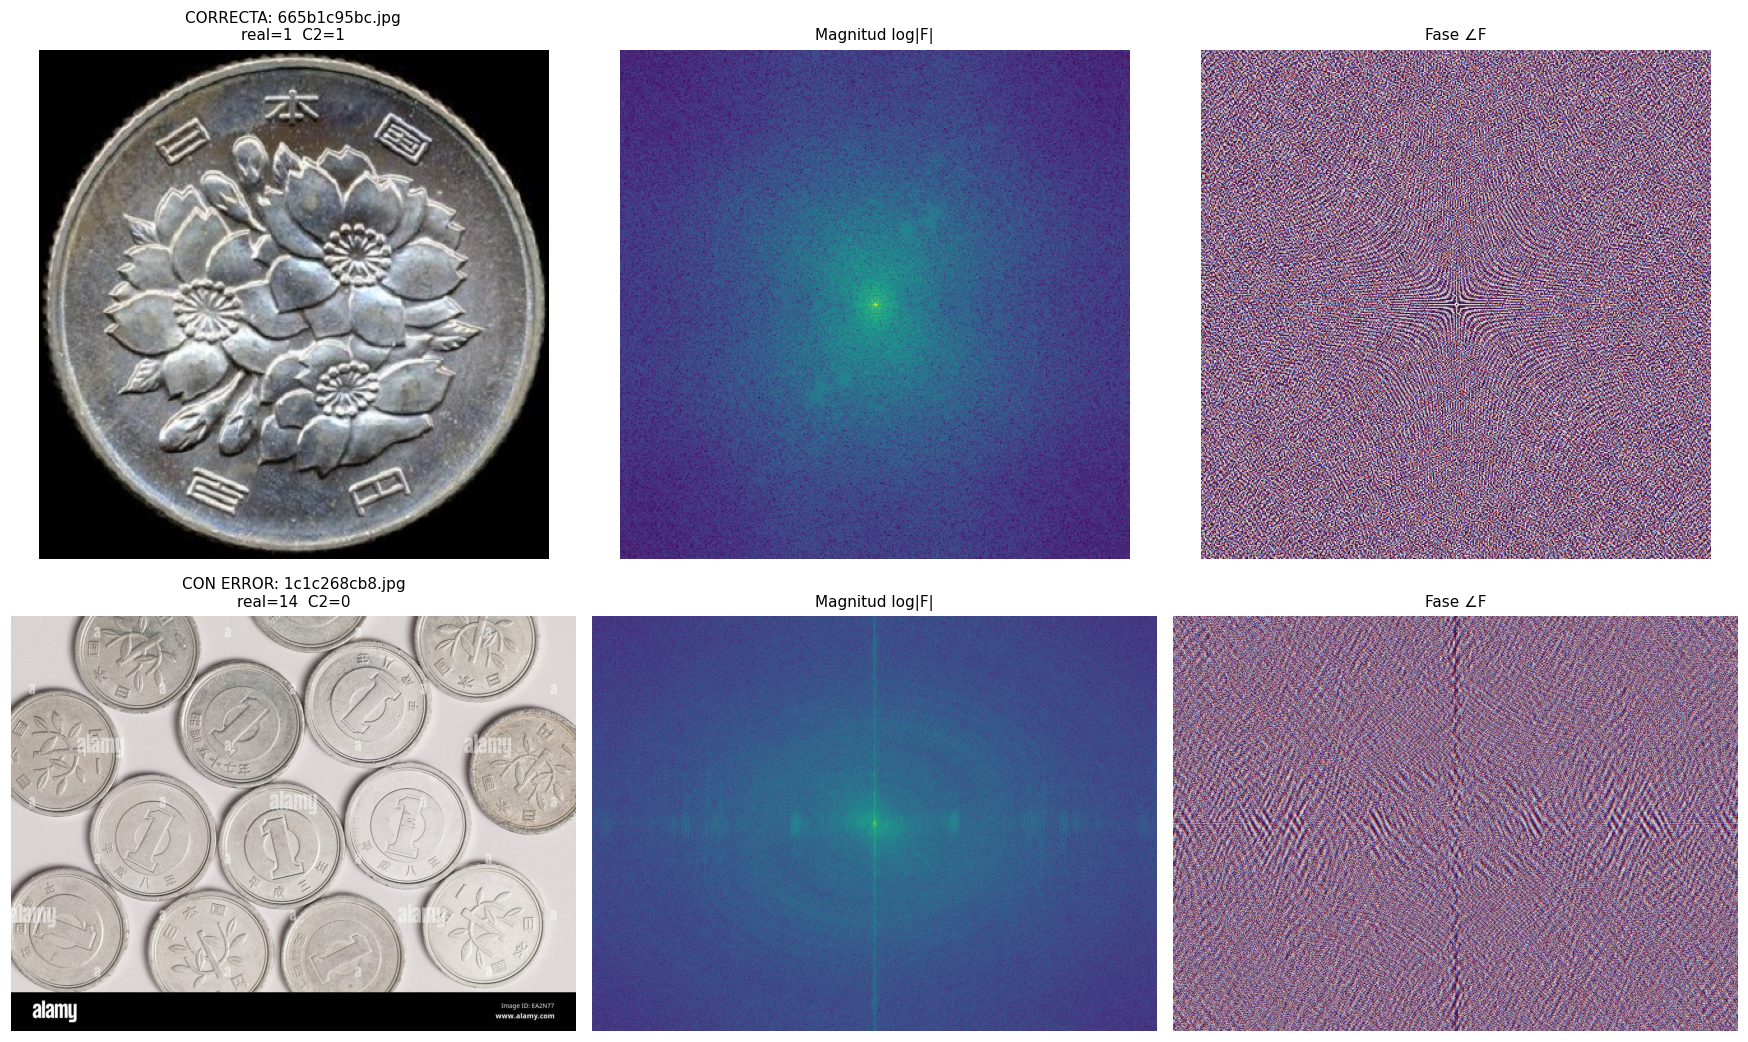
\includegraphics[width=0.86\linewidth]{figs/fourier.png}
\caption{Imagen original, magnitud ($\log|F|$) y fase del espectro de Fourier, para un caso correcto
(arriba) y uno con error (abajo).}
\label{fig:fourier}
\end{figure}

\begin{figure}[ht]
\centering
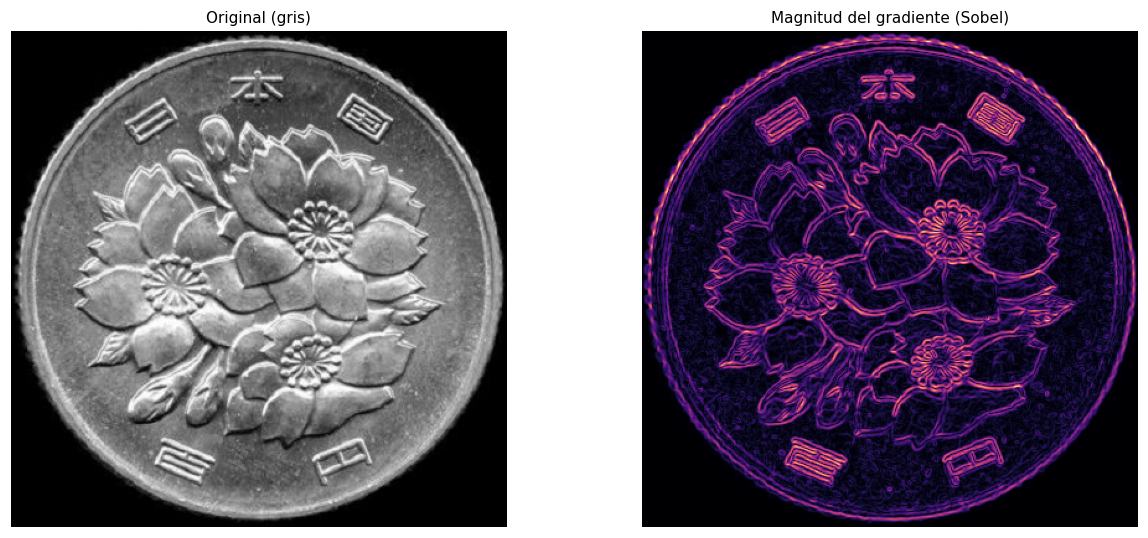
\includegraphics[width=0.78\linewidth]{figs/sobel.png}
\caption{Realce de bordes mediante convolución con el \emph{kernel} de Sobel: los bordes de las monedas
corresponden a las altas frecuencias del espectro.}
\label{fig:sobel}
\end{figure}

\subsection{Ablación y sensibilidad (Parte VII)}

La Tabla~\ref{tab:abl} elimina/modifica un componente a la vez (partiendo de C2) y la
Figura~\ref{fig:sens} barre el radio del disco morfológico.

\begin{table}[ht]
\centering
\caption{Estudio de ablación sobre C2.}
\label{tab:abl}
\begin{tabular}{lcc}
\hline
Variante & MAE & Exactas (\%) \\
\hline
A0 baseline (C2)        & 1.69 & 42.3 \\
A1 sin gamma            & 1.50 & 50.0 \\
A2 sin suavizado        & 1.96 & 42.3 \\
A3 sin morfología       & 2.08 & 53.8 \\
A4 sin filtro excentr.\ & 1.65 & 42.3 \\
\hline
\end{tabular}
\end{table}

\begin{figure}[ht]
\centering
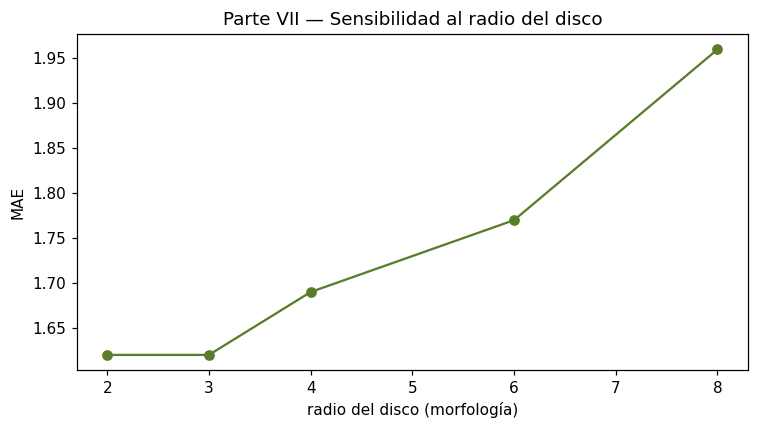
\includegraphics[width=0.62\linewidth]{figs/sensibilidad.png}
\caption{Sensibilidad del MAE al radio del disco morfológico.}
\label{fig:sens}
\end{figure}

% ====================== 4. ANALISIS ======================
\section{Análisis y discusión de resultados}

\textbf{Desempeño global.} La configuración \textbf{C3 (k-means)} obtiene el mejor resultado (MAE $1{,}50$;
$50\%$ de conteos exactos), aunque la diferencia con C1/C2 es pequeña: las tres rondan un MAE de
$1{,}5$--$1{,}7$ monedas. Esto es coherente con la teoría: el k-means segmenta usando los tres canales de
color, por lo que separa la moneda del fondo incluso cuando ambos tienen brillo parecido, situación en la
que el umbral global de Otsu (C1/C2) se degrada.

\textbf{Causas de éxito y fracaso.} Los aciertos corresponden a escenas con monedas separadas y buen
contraste, donde cada moneda produce una región redonda (baja excentricidad). Los fallos tienen dos
orígenes opuestos: \emph{subconteo} cuando las monedas se tocan (sus regiones se fusionan en un blob
alargado que el filtro de excentricidad puede incluso descartar) y errores en escenas oscuras o con
reflejos, donde Otsu deja máscaras incompletas. El método es sólido para conteos bajos y se degrada con la
densidad y el solapamiento.

\textbf{Práctica vs.\ teoría (espacio--frecuencia).} Los espectros confirman lo esperado: la energía se
concentra en el centro (bajas frecuencias = fondo y cuerpo de las monedas), mientras que los bordes
---resaltados por el filtro de Sobel--- aportan altas frecuencias en la periferia. La imagen con error
exhibe más energía dispersa en altas frecuencias (reflejos, textura, recortes y contactos), justo los
elementos que confunden al umbral y al etiquetado. Así, la dificultad observada en el dominio espacial se
manifiesta como contenido de alta frecuencia.

\textbf{Lectura honesta de la ablación.} La Tabla~\ref{tab:abl} permite distinguir mejoras reales de
aparentes:
\begin{itemize}
\item \emph{Morfología} (A3): su eliminación es lo más dañino (MAE $1{,}69\rightarrow2{,}08$); es la
columna vertebral de la limpieza de la máscara.
\item \emph{Suavizado} (A2): también \textbf{ayuda} ---quitarlo sube el MAE a $1{,}96$--- porque atenúa
ruido y reflejos.
\item \emph{Gamma} (A1): en cambio \textbf{no ayuda aquí}; quitarlo \emph{mejora} el MAE ($1{,}50$). El
$\gamma=0{,}4$ del ejemplo de clase estaba ajustado a \emph{su} imagen oscura; en las yen no es necesario.
Es la típica ``mejora aparente'' que la ablación desenmascara.
\item \emph{Filtro de excentricidad} (A4): efecto \textbf{ambivalente}; ayuda a rechazar fusiones pero
también descarta monedas recortadas (alargadas) en el borde.
\item \emph{Radio del disco}: el MAE crece con el radio; un disco pequeño (2--3) limpia lo suficiente y los
discos grandes fusionan monedas vecinas.
\end{itemize}

\textbf{Discusión técnica (Parte VI).}
\emph{(1) Dificultades:} la heterogeneidad del dataset (resolución de dos órdenes de magnitud, iluminación
de oscura a saturada, monedas en contacto). \emph{(2) Decisión de mayor impacto:} el etiquetado de
componentes sobre una buena máscara morfológica y el reescalado de las imágenes grandes para que los
parámetros sean comparables. \emph{(3) Hipótesis incorrectas:} se esperaba que el gamma del ejemplo de
clase ayudara siempre (no es así en yen) y que el filtro de excentricidad mejorara siempre (es ambivalente).
\emph{(4) Conceptos del curso que ayudaron:} realce de intensidad, Otsu, morfología, \code{label}/
\code{regionprops}, k-means y Fourier 2D. \emph{(5) Mejoras futuras:} umbral local/adaptativo, separación
de monedas en contacto y estimación automática del radio típico por imagen. \emph{(6) ¿Bastan las técnicas
clásicas?} Para escenas controladas, sí (interpretables y rápidas); para el caso general (solapamiento,
fondos complejos, iluminación adversa) alcanzan un techo y dependen del ajuste de parámetros: una solución
robusta de propósito general requeriría complementarlas con aprendizaje, usando lo clásico como
preprocesamiento.

% ====================== 5. CONCLUSIONES ======================
\section{Conclusiones}

Se construyó un sistema de conteo de monedas yen empleando \emph{exclusivamente} los métodos del curso: el
pipeline del profesor (\code{rgb2gray}+gamma $\rightarrow$ Otsu $\rightarrow$ morfología $\rightarrow$
\code{measure.label} $\rightarrow$ \code{regionprops} por área y excentricidad $\rightarrow$ bounding
boxes), con k-means como segunda segmentación y Fourier 2D para el análisis espacio--frecuencia. La
configuración con k-means y un esquema de componentes simple quedan parejos (MAE $\approx 1{,}5$). La
ablación mostró que la \textbf{morfología y el etiquetado} son la columna vertebral, que el \textbf{suavizado
ayuda}, y que el \textbf{gamma del ejemplo de clase} y el \textbf{filtro de excentricidad} no aportan o son
ambivalentes en este conjunto. El análisis de Fourier confirmó la correspondencia entre la dificultad
espacial y el contenido de alta frecuencia. En síntesis, las técnicas clásicas bastan para escenas
controladas pero tienen un techo claro ante el solapamiento y la iluminación adversa, y conviene validar
cada ``mejora'' con evidencia antes de incorporarla.

% ====================== USO DE IA ======================
\section*{Uso de herramientas de Inteligencia Artificial}
\addcontentsline{toc}{section}{Uso de herramientas de Inteligencia Artificial}

\textbf{1. Herramientas.} Un asistente de IA basado en LLM como apoyo de programación y redacción, la
documentación de scikit-image/scikit-learn/SciPy y, sobre todo, los \textbf{Colabs del propio curso}.

\textbf{2. Cómo se usaron.} Para estructurar el código, recordar firmas de funciones
(\code{measure.regionprops}, \code{KMeans}, \code{scipy.fft.fft2}) y depurar. Las decisiones metodológicas
---usar solo métodos vistos en clase, curar el subconjunto limpio de yen, qué configuraciones comparar y
cómo diseñar la ablación--- y la interpretación de los resultados fueron propias.

\textbf{3. Aportes útiles.} Acelerar el andamiaje del código y recordar el patrón
\code{label}$\rightarrow$\code{regionprops}$\rightarrow$\code{bbox} del profesor.

\textbf{4. Recomendaciones incorrectas o incompletas.} En una primera versión la IA propuso
\textbf{watershed, Hough y CLAHE}, técnicas que \emph{no} se revisaron en clase; al contrastar con los
Colabs del curso se reemplazaron por el método real del profesor. También sugirió \textbf{parámetros
absolutos en píxeles} que fallan por la variación de resolución (se corrigieron reescalando) y algunas
imágenes que eran en realidad \textbf{miniaturas con texto} (se descartaron tras revisarlas).

\textbf{5. Verificación de la calidad.} Ejecutando el notebook completo (0 errores), comparando contra el
conteo real, revisando visualmente máscaras y \emph{bounding boxes}, y contrastando cada técnica con el
Colab de la clase que la introduce. Cuando una recomendación contradecía la evidencia, prevaleció la
evidencia.

% ====================== 6. REFERENCIAS ======================
\begin{thebibliography}{9}
\bibitem{gw} R.\ C.\ Gonzalez y R.\ E.\ Woods, \emph{Digital Image Processing}, 4.\textsuperscript{a} ed.,
Pearson, 2018.
\bibitem{skimage} Documentación de \textbf{scikit-image} --- \code{morphology}, \code{measure.label},
\code{measure.regionprops}, \code{filters.threshold\_otsu}. \url{https://scikit-image.org/}
\bibitem{sklearn} Documentación de \textbf{scikit-learn} --- \code{cluster.KMeans}.
\url{https://scikit-learn.org/}
\bibitem{scipy} Documentación de \textbf{SciPy} --- \code{scipy.fft} (\code{fft2}, \code{fftshift}),
\code{scipy.signal.convolve2d}. \url{https://scipy.org/}
\bibitem{otsu} N.\ Otsu, ``A Threshold Selection Method from Gray-Level Histograms'', \emph{IEEE TSMC},
1979.
\bibitem{colabs} Colabs del curso \textbf{PDDI (UTEM)} --- Clases 15 (k-means), 16 (conteo de monedas,
morfología, \code{regionprops}; convolución/bordes) y 05--10 (Fourier).
\end{thebibliography}

\end{document}
